\documentclass[french]{tccv}
\usepackage[hmargin=0.2cm,vmargin=0cm]{geometry}
\usepackage{amsfonts} 								% for the \checkmark command 
\usepackage[framemethod=TikZ]{mdframed}						% For box around text

\usepackage[overlay,absolute]{textpos}
\setlength{\TPHorizModule}{1cm}
\setlength{\TPVertModule}{1cm}

\usepackage{fontspec}




\mdfsetup{
   middlelinecolor=mybluegrey,
   middlelinewidth=2pt,
   backgroundcolor=white!0,
   roundcorner=10pt,
   skipabove=0,
   fontcolor=black,
}

\fontdir[fonts/]
\colorlet{awesome}{awesome-skyblue}


\begin{document}
%%%%%%%%%%%%%%%%%%%%%%%%%%%%%%%%%%%%%%%%%%%%%%%%%%%%%%%%%%%%%%%%%%%%%%%%%%%%%%%%%%%%%%%%%%%%%%%%%%%%%%%%%%%%%%%%%%%%


\begin{textblock}{6.5}(0.5,0.5)
\personal
    []
    {16 Rue Chicogné, 35000 Rennes}
    {+33 07 83 88 33 32}
    {r.sanhuezarepetto@gmail.com}
\end{textblock}

\begin{textblock}{10}(8.0,1)
      \headerfirstnamestyle{Roc\'io}   \headerlastnamestyle{Sanhueza}
\end{textblock}

\begin{textblock}{21}(17.5,0.5)
		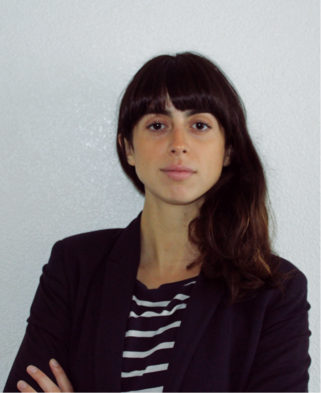
\includegraphics[width=3cm]{../Figure/Rocio3.png}
\end{textblock}  









\begin{textblock}{7}(0.5,4)
\begin{mdframed}

\section{Éducation}
\begin{yearlist}

\item[Master 1 Science politique]{2015 -- 2016}
     {Université de Rennes 1}
     {Enseignements suivis: pensée politique contemporaine, 
     régimes contemporaines, sociologie de la communication, pensée sociologique, 
     Appro\-ches de l'Union Européen, Grand dossiers de\- l'ad\-mi\-ni\-stra\-tion.}




\item[Diplôme en Communication sociale et journalisme (Bac+5)]{2008 -- 2013}
     {Universidad de Santiago de Chile}
     {Spécialité politique
     Mention très bien
     }

     
\item[Échange universitaire -- journalisme]{2011 -- 2011}
     {Universidade Estadual Pau\-li\-sta }
     {Enseignements suivis: réalité socio - économique et politique brésilienne. \\
     Langue portugaise: littérature, sémiotique, stratégies de communication publique}


\end{yearlist}
\end{mdframed}


\begin{mdframed}
\section{Compétences linguistiques}

\begin{factlist}
\item{Espagnol} {Langue maternelle}	
\item{Français} {Courant}	
\item{Anglais}  {Niveau B2}	
\item{Portugais}{Niveau B2}
\end{factlist}

\section{Logiciels}
\descriptionstyle{
Environnement PC et Linux,
Pack office et Libre office,
Adobe Photoshop, Premiere, \\
%Python, 
Gimp,
HTML5,
\LaTeX.
}


\section{Aptitudes}
\descriptionstyle{
  \checkmark Aisance communicationnelle et relationnelle \\
  \checkmark Disciplinée et organisée \\
  \checkmark Esprit d'équipe \\  
}



%%%%%%%%%%%%%%%%%%%%%%%%%%%%%%%%%%%%%%%%%%%%%%%%%%%%%%%%%%%%%%%%%%%%%%%%%%%%%%%%%%%%%%%%%%%%%%%%%%%%%%%%%%%%%%%%%%%%%%%%%%%%%%%%%%%%%%%%%%
%&
\end{mdframed}
\end{textblock}


\mdfsetup{middlelinecolor=white!0}

\begin{textblock}{13}(7.7,4)
\begin{mdframed}
\section{Expérience Professionnelle}


\begin{eventlist}
\item{Avril 2014 -- Mars 2015}
     {Sénat du Chili}
     {Conseillère en communication et attachée de presse}
     \descriptionstyle{ 
     Contexte : Le cabinet politique du sénateur Felipe Harboe cherche continuement améliorer sa visibilité et présence dans les médias \\ 
     Missions : 
     }  

  \setlength{\parskip}{-10pt}
    \begin{itemize}
      \setlength\itemsep{-3pt} 
      \cvitem[\checkmark]  \descriptionstyle{ Mise en œuvre des actions de communication et des relations avec la presse                     }
      \cvitem[\checkmark]  \descriptionstyle{ Rédaction des articles, communiqués et dossiers de presse. Supervision des interviews avec les médias      }
      \cvitem[\checkmark]  \descriptionstyle{ Organisation de conférences de presse                                                                                               }
      \cvitem[\checkmark]  \descriptionstyle{ Administration de réseaux sociaux                                                    }
    \end{itemize}     
     \descriptionstyle{ 
    Résultats : Présence constante dans la presse nationale et régionale  \\
               Entre 600 et 1100 visites quotidiennes sur le site web 
      }
               
\item{Mai 2013 -- Déc. 2014}
     {Aluro 35, Santiago, Chili}
     {Productrice générale}
     
          \descriptionstyle{ 
Contexte : La maison de production indépendante Aluro 35 doit produire le programme culturel de télévision La Bicicleta transmit par la chaîne 13C \\
Missions :
     }  
     
    \begin{itemize}
      \setlength\itemsep{-3pt} 
      \cvitem[\checkmark] \descriptionstyle{ Gestion des rapports avec la chaîne et négociation de budgets                          }
      \cvitem[\checkmark] \descriptionstyle{ Préparation du lieu de tournage, mobilisation et interviews. Aide à la préparation du contenu des entretiens   }
      \cvitem[\checkmark] \descriptionstyle{ Administration de réseaux sociaux et animation de communautés (Facebook, Twitter, Instagram)                                                 }
      \cvitem[\checkmark] \descriptionstyle{ Création du dossier de presse pour les lancements du programme                                                   }

    \end{itemize}     
   \descriptionstyle{  
Résultats: Renouvellement d'une deuxième saison avec plus de sponsors \\
Montée de la visibilité des artistes et associations culturels interviewés \\
Obtention d’un fond public du Ministère de Culture pour une troisième saison  \\
     }
     
     
\item{Oct. 2013 -- Fév. 2014 }     
  {Más comunicaciones, Santiago, Chili}     
  {Journaliste}
          \descriptionstyle{ 
Contexte : L’agence Mas comunicaciones doit en permanence améliorer la communication globale et la présence dans les médias
pour des marques comme Dole, Artilec, MOR et Flores\\
Missions :
     }  

\begin{itemize}
      \setlength\itemsep{-3pt} 
      \cvitem[\checkmark] \descriptionstyle{ Préparation d'articles pour les médias                                            }
      \cvitem[\checkmark] \descriptionstyle{ Création de dossiers de presse                                                     }
      \cvitem[\checkmark] \descriptionstyle{ Ciblage des journalistes spécialisés et amélioration de la basse de donnés  }
\end{itemize}       
   \descriptionstyle{  
Résultats: Présence constante dans la presse nationale (El Mostrador; revues Paula, Mujer, Vanidades, Ya) et regionale (El Rancaguino) 
     }


\item{Avril 2012 -- Avril 2013 }     
  {Killahue corporation, Santiago, Chili}     
  {Chargée de projet}

          \descriptionstyle{ 
Contexte : Projet innovateur qui cherche à urbaniser un secteur rural du Chili, tout en préservant son milieu naturel et le développement de leurs habitants \\
Missions :
     }    
  
\begin{itemize}
      \setlength\itemsep{-3pt} 
      \cvitem[\checkmark]  \descriptionstyle{ Recherche des informations juridiques et environnementales de projets similaires                  }
      \cvitem[\checkmark]  \descriptionstyle{ Gestion et coordination de réunions, plus la préparation de matériaux visuels et écrits    }
      \cvitem[\checkmark]  \descriptionstyle{ Administration de réseaux sociaux                                                                                                            }
      \cvitem[\checkmark]  \descriptionstyle{ Formalisation et rédaction du travail réalisé et des décisions pris dans l’ensemble des réunions                                             }

\end{itemize}      
   \descriptionstyle{  
Résultats: Définition de l’image corporatif \\
Identification des problématiques internes de la corporation et production des solutions \\
Amélioration du niveau de présence dans les médias spécialisés \\
     }

  
  


   


\end{eventlist}


\end{mdframed}
\end{textblock}
\end{document}
